%%%%%%%%%%%%%%%%%%%%%%% file template.tex %%%%%%%%%%%%%%%%%%%%%%%%%
%
% This is a template file for Web of Conferences Journal
%
% Copy it to a new file with a new name and use it as the basis
% for your article
%
%%%%%%%%%%%%%%%%%%%%%%%%%% EDP Science %%%%%%%%%%%%%%%%%%%%%%%%%%%%
%
%%%\documentclass[option comma separated list]{webofc}
%%%Three important options:
%%% "epj" for EPJ Web of Conferences Journal
%%% "bio" for BIO Web of Conferences Journal
%%% "mat" for MATEC Web of Conferences Journal
%%% "itm" for ITM Web of Conferences Journal
%%% "e3s" for E3S Web of Conferences Journal
%%% "shs" for SHS Web of Conferences Journal
%%% "twocolumn" for typesetting an article in two columns format (default one column)
\documentclass[epj,twocolumn]{webofc}
\usepackage[varg]{txfonts}   % Web of Conferences font
%
% Put here some packages required or/and some personnal commands
%
% Important: please activate and fill the "wocname" command with the exact title of the series for conferences not included in any of the series listed on the top
\usepackage{siunitx}
\usepackage{cleveref}
\usepackage{subcaption}
\captionsetup{compatibility=false}

% Very important: please fill the "woctitle" command with the exact title of the conference
%
\woctitle{Powders \& Grains 2017}
%
%
\begin{document}
%
\title{Collapse of tall granular columns in fluid}
%
% subtitle is optionnal
%
%%%\subtitle{Do you have a subtitle?\\ If so, write it here}

\author{\firstname{Krishna} \lastname{Kumar}\inst{1}\fnsep\thanks{\email{kks32@cam.ac.uk}} \and
        \firstname{Kenichi} \lastname{Soga}\inst{2}\fnsep\thanks{\email{soga@berkeley.edu}} \and
        \firstname{Jean-Yves} \lastname{Delenne}\inst{3}\fnsep\thanks{\email{delenne@supagro.inra.fr}}
}

\institute{Department of Engineering, University of Cambridge, UK 
\and
           University of California, Berkeley, USA
\and
            INRA, CIRAD, University Montpellier 2 and SupAgro, France
}

\abstract{%
  Avalanches, landslides, and debris flows are geophysical hazards, involve
  rapid mass movement of granular solids, water, and air as a multi-phase
  system. In order to describe the mechanism of immersed granular flows,
  it is important to consider both the dynamics of the solid phase and the
  role of the ambient fluid. In the present study,
  the collapse of a granular column in fluid is
  studied using 2D LBM - DEM. The flow kinematics are compared with the dry
  and buoyant granular collapse to understand the influence of hydrodynamic
  forces and lubrication on the run-out. In the case of tall columns,
  the amount of material destabilised above the failure plane is larger than
  that of short columns. Hence in tall columns, the surface area of the
  mobilised mass that interacts with the surrounding fluid is significantly
  higher than the short columns. This increase in the area of soil - fluid
  interaction results in an increase in the formation of turbulent vortices
  that alter the deposit morphology during the collapse. It is observed that
  the vortices result in the formation of heaps that significantly affect
  the distribution of mass in the flow. In order to understand the behaviour
  of tall columns, the run-out behaviour
  of a dense granular column with an initial aspect ratio of 6 is studied.
  The collapse of a tall granular column on slopes of 0, 2.5, 5 and 7.5
  are studied.}
%
\maketitle
%
\section{Collapse of granular columns}
The collapse of a granular column on a horizontal surface is a simple case
of granular flow, however a proper model that describes the flow dynamics
is still lacking. Experimental investigations have shown that the flow
duration, the spreading velocity, the final extent of the deposit, and the
energy dissipation can be scaled in a quantitative way independent of
substrate properties, grain size, density, and shape of the granular
material and released mass
~\cite{Topin2011, Staron2007a, Lajeunesse2005, Lube2005}. 

Granular collapse on a horizontal plane exhibit two distinct flow regimes:
(a) for columns with aspect ratio ‘a’ < 1.7 a linear relation between the
spread and aspect ratio can be observed, and (b) for ‘a’ > 1.7 a power-law
relationship exists. A simple frictional dissipation model is able to
capture the flow dynamics for columns with small aspect ratios
~\cite{soundararajan2015}. However, for tall columns the flow
dyanmics is controlled by the initial collisional regime, resulting in a
power-law relationship with the aspect ratios. Simple mathematical models
based on conservation of horizontal momentum capture the scaling laws of
the final deposit, but fail to describe the initial transition regime
~\cite{Kumar2012}. Granular flow is modelled as a frictional dissipation
process in continuum mechanics but the lack of influence of inter-particle
collision and friction on the energy dissipation and spreading dynamics is
surprising.

The amount of material destabilised above the failure plane, in tall columns,
is larger than that of short columns. This increase in the mobilised mass
results in a signficant increase in the surface area of granular mass that
interacts with the surrounding fluid. The increase in the area of soil -
fluid interaction results in an increase
in the formation of turbulent vortices that alter the deposit morphology during 
the collapse. It is observed that the vortices result in formation of heaps 
that significantly affect the distribution of mass in the flow.
The distribution of mass in a granular flow plays a crucial role in the
flow kinematics~\cite{Staron2007a}. In order to understand the
behaviour of tall columns, the run-out behaviour of a dense granular column
with an initial aspect ratio of 6 is studied using Lattice Boltzmann - Discrete
Element Method coupling.

\section{LBM-DEM coupling}
The Lattice Boltzmann Method (LBM) is an alternative approach to
the classical Navier-Stokes solvers for fluid flow and works on an
equidistant grid of cells, called lattice cells, which interact only with
their direct neighbours~\cite{He1997}. The fluid domain is divided into
a rectangular grid or lattice, with the same spacing ‘h’ in both the x-
and the y-directions. The present study focuses on 2-D problems; hence,
the D2Q9 momentum discretization is adopted, where the fluid particles at
each node are allowed to move to their eight immediate neighbours
with eight different velocities $\mathit{e_i} (\mathit{i}=1\,,\dots\,,8)$.
The primary variables in LB formulation are called the \textit{fluid 
density distribution functions}, $\mathit{f_i}$, each representing the probable 
amount of fluid particles moving with the velocity $\mathit{e_i}$ along the 
direction $\mathit{i}$ at each node. In the present study, Lattice-Boltzmann
- Multiple Relaxation Time (LBM-MRT) is used for numerical stability.
The nine eigen values of $\mathbf{S}$ are all between 0 and 2 so as to
maintain linear stability and the separation of scales. In  this  study,
the Large Eddy Simulation (LES) is adopted to solve for turbulent flow
problems. The separation of scales is achieved by filtering of the
Navier-Stokes equations, from which the resolved scales are directly
obtained and unresolved scales are modelled by a one-parameter
Smagorinski sub-grid methodology.%~\cite{Smagorinsky1963}. 

Lattice Boltzmann approach can accommodate large grain sizes and the
interaction between the fluid and the moving grains can be modelled
through relatively simple fluid – grain interface treatments. Further,
employing the Discrete Element Method (DEM) to account for the
grain – grain interaction naturally leads to a combined LB – DEM
procedure~\cite{Kumar2012}. The Eulerian nature of the LBM formulation,
together with the common explicit time step scheme of both LBM and DEM
makes this coupling strategy an efficient numerical procedure for the
simulation of grain – fluid systems. A no-slip boundary condition is
used to simulate grain – fluid and grain – grain interactions. The
solid grains inside the fluid are represented by lattice
nodes. The discrete nature of lattice, results in a stepwise
representation of the surfaces, which are circular, hence
sufficiently small lattice spacing is adopted. In order to model flow
through interconnected pore space, a reduction in radius (The
hydrodynamic radius \textit{r}) is assumed during the
LBM computation~\citep{soundararajan2015}.

\section{Numerical set-up}
In this study, a 2D poly-disperse system ($d_{max} / d_{min} = 1.8$) of
circular discs in fluid was used to understand the behaviour of granular
flows on slopes (see~\cref{fig:geometry}).
The soil column was modelled using 2500 discs of density
2650~\si{\kilogram\per\meter\cubed} and a contact friction angle of
26\si{\degree}.  The  collapse of the column was simulated inside a fluid
with a density of 1000~\si{\kilogram\per\meter\cubed} and a kinematic viscosity
of $1 \times 10^{-6}$~\si{\meter\squared\per\second}. The fluid was modelled
with 5 to 9 million LB nodes. GPU computing was used to simulate the problem.
The choice of a 2D geometry has the advantage of cheaper computational
effort than a 3D case, makeing it feasible to simulate very large systems.
A granular column of aspect ratio `\textit{a}' of 6 was used. A hydrodynamic
radius of \textit{r} = 0.85 \textit{R} is adopted. Dry analyses were also
performed to study the effect of hydrodynamic forces on the run-out distance.
The collapse of a tall granular column on slopes of 0\si{\degree},
2.5\si{\degree}, 5\si{\degree} and 7.5\si{\degree} are studied.

\begin{figure}
  \centering
  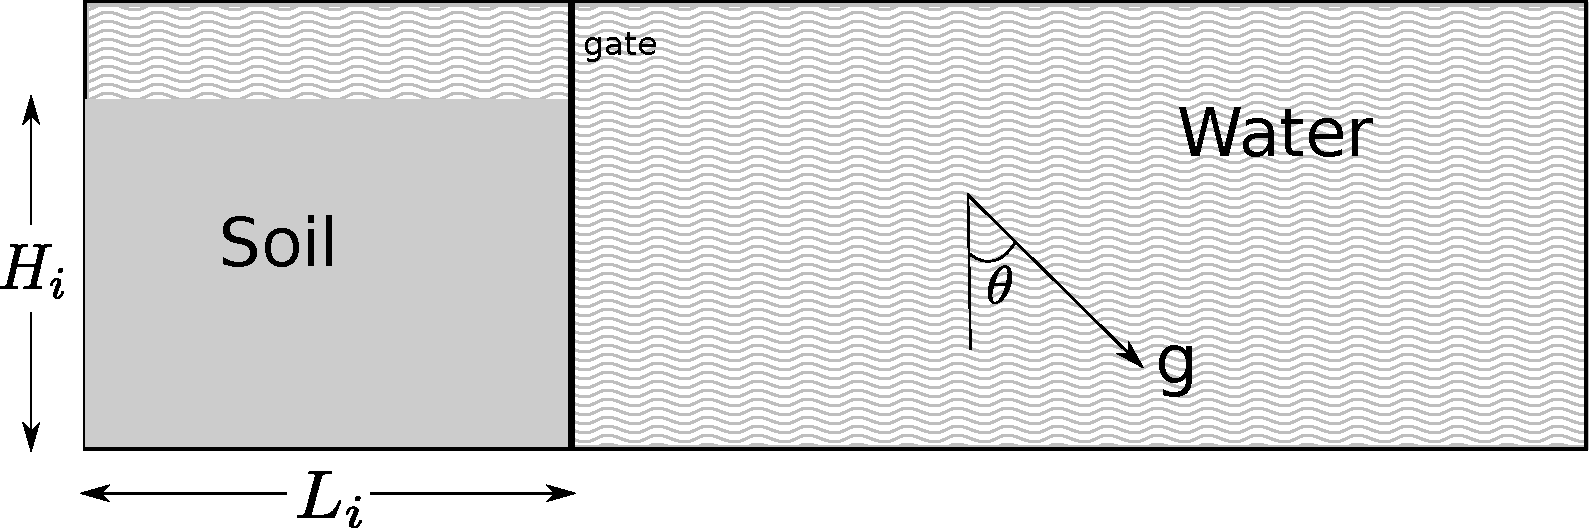
\includegraphics[width=0.95\linewidth]{figs/geometry}
  \caption{Underwater granular collapse set-up.
    The slope angle is represented by $\theta$.}
  \label{fig:geometry}
\end{figure}

\section{Collapse on a horizontal plane}
Snapshots of the collapse of an aspect ratio 6 column in fluid on a horizontal 
surface are shown in~\cref{fig:LBM_DEM_a6}. The initial stage of collapse is 
characterised by the free-fall of grains above the failure surface.
The height of the static region, which is below the shear-failure surface,
is shorter than the total height of the column. As the grains experience
free-fall they interact with the surrounding fluid. Unlike the dry condition,
as the grains undergo free-fall due to gravity, they interact 
with the surrounding fluid experiencing drag forces. This results in a 
significant drop in the kinetic energy available for the flow.
However, no vortices are observed during the initial stage of collapse.

\begin{figure}[htpb]
\centering
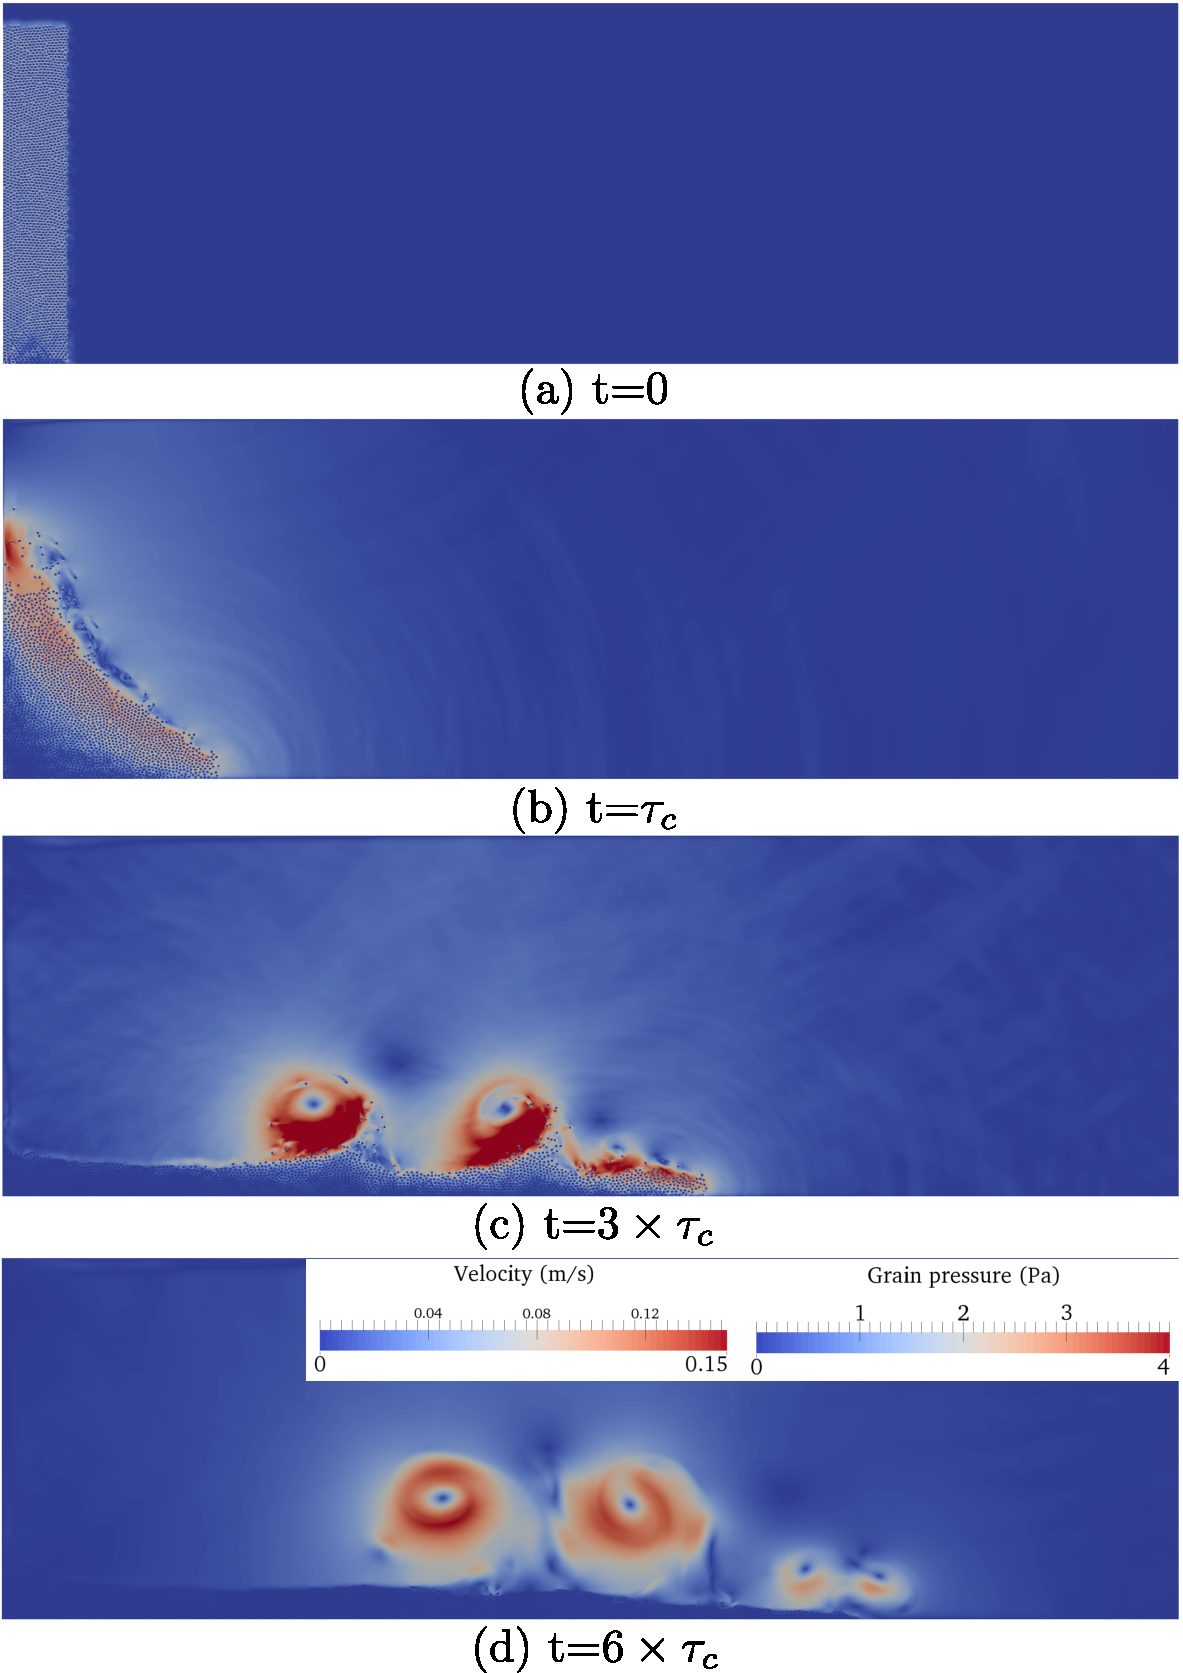
\includegraphics[width=0.9\linewidth]{figs/lbm_dem_a6}
\caption{Flow evolution of a granular column collapse in fluid (a = 6) on a 
horizontal surface.}
\label{fig:LBM_DEM_a6}
\end{figure}

As the grains reach the static region, they interact with the neighbouring
grains and the kinetic energy gained during the free fall is converted into
horizontal acceleration. Uniquely during this stage ($t = 3\tau_c$) the
interactions between the soil grains on the surface with the surrounding
fluid result in the formation of eddies. The number of eddies formed during
the flow is proportional to the surface area of the granular mass interacting
with the fluid. Hydroplaning can be observed at the flow front ($t = 3\tau_c$).
Two large vortices with almost the same size can be observed at the final stage of 
collapse. The soil grains on the surface experience suction due to formation of 
eddies and this results in formation of heaps of granular mass in front of each 
vortex. Unlike short columns, these vortices have 
a significant influence on the mass distribution along the run-out. Heaps of 
granular material can be observed in front of each vortex. The number of 
vortices formed during a collapse is found to be proportional to the amount of 
material destabilised, i.e., the length of free-surface interacting with the 
fluid influences the number of vortices generated during the collapse. The 
reappearance of force chains at $t = 6\tau_c$ indicates the 
granular mass is consolidating resulting in an increase in the shear strength. 
The formation of heaps, although in evidence, doesn't significantly 
affect the distribution of mass in the case of collapse on a horizontal plane. 



\section{Collapse on slopes}
Snapshots of the collapse of a granular column (\textit{a} = 6) on a inclined 
plane at angle of 5\si{\degree} are shown in~\cref{fig:a6_slope_snapshots}. 
The collapse on a slope of 5\si{\degree} show flow evolution behaviour similar 
to the case of collapse on a horizontal plane. The vortices are formed only 
during the horizontal spreading stage $t = 3\tau_c$, but the number of vortices 
formed during the collapse is more than the collapse on a horizontal plane. 
However, as the flow progresses a single large vortex engulfs other smaller 
vortices, thus having a significant influence on the mass 
distribution.

\begin{figure}[!h]
\centering
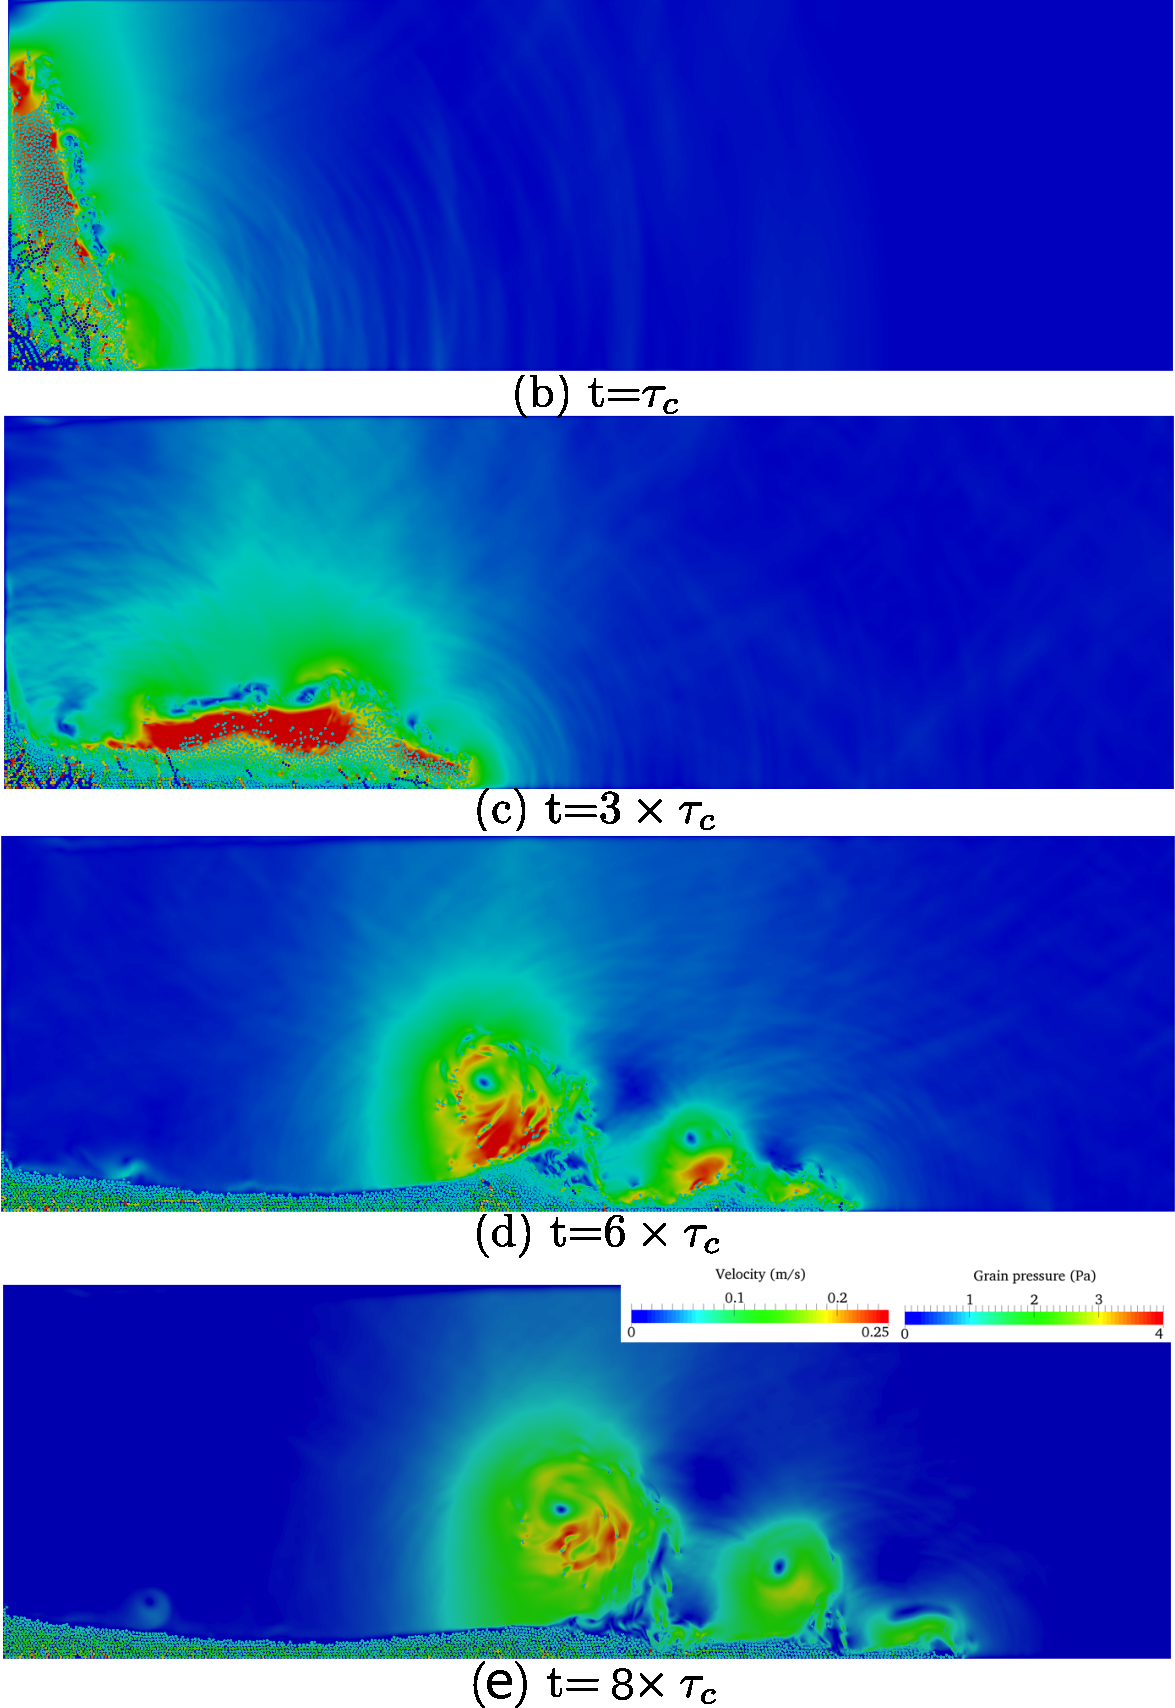
\includegraphics[width=0.9\linewidth]{figs/lbm_dem_a6_slope5}
\caption[Flow evolution of a granular column collapse in fluid (a = 6) on a 
slope of 5\si{\degree}]{Flow evolution of a granular column collapse in fluid 
(a = 6) on a slope of 5\si{\degree}. Shows the velocity profile of fluid due to 
interaction with the grains (red - higher velocity).}
\label{fig:a6_slope_snapshots}
\end{figure}

~\Cref{fig:a6_slope_voro} shows 
the distribution of mass and the packing density at $t = 6\tau_c$ and
$t = 8\tau_c$. A heap can be observed in front of the large vortex almost at the 
middle of the flow. The height of the heap formed in the middle of the granular 
flow is higher than the collapse height next to the wall. However, when the 
flow comes to rest and the vortex moves 
away from the flowing surface, the mass present in the heap gets redistributed 
(as seen at $t = 8\tau_c$). This behaviour is significantly different from that 
observed in the case of short columns. More denser packing can be observed in front
of the eddies, resulting in spectrums dense - loose regions.

\begin{figure}
\makebox[\linewidth][c]{
\begin{subfigure}[b]{0.95\linewidth}
	\centering
    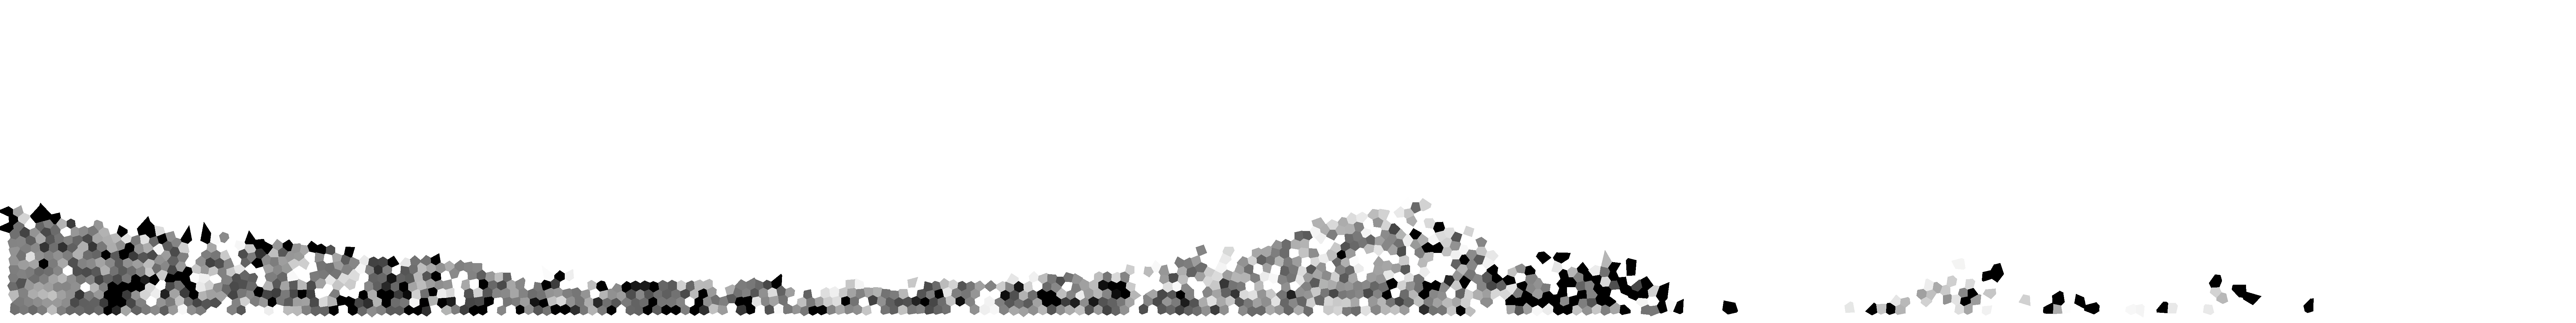
\includegraphics[width=0.95\linewidth]{figs/a6_slope5_6tc}
    \caption*{$t = 6\tau_c$}
    \label{fig:a6_slope5_6tc}
\end{subfigure}
}\\
\makebox[\linewidth][c]{
\begin{subfigure}[b]{0.95\linewidth}
	\centering
    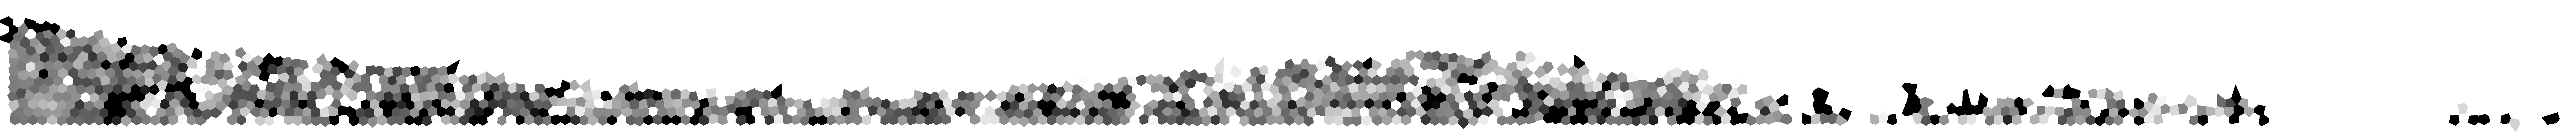
\includegraphics[width=0.95\linewidth]{figs/a6_slope5_8tc}
    \caption*{$t = 8\tau_c$}
    \label{fig:a6_slope5_8tc}
\end{subfigure}
}
\caption{Packing density of a granular column collapse in fluid (a = 6) on a 
slope of 5\si{\degree}.}
\label{fig:a6_slope_voro}
\end{figure}

\subsection{Effect of slope angle}
In order to understand the influence of slope angles on the run-out behaviour, 
the collapse of a granular column with an initial aspect ratio of 6 is 
performed on slopes of 0\si{\degree}, 2.5\si{\degree}, 5\si{\degree} and 
7.5\si{\degree}. The run-out evolution with time for different slope angles are 
presented in~\cref{fig:Runout_a6_slope}. The run-out distance increases with 
increase in the slope angle, however the run-out distance in the fluid is 
significantly shorter than the dry condition. The slow evolution of run-out in 
the submerged condition is due to the delay in the dissipation of large 
negative pore-pressures developed during the initial stage of the collapse. The 
formation of eddies during the flow indicates that most of the potential energy 
gained during the free-fall is dissipated through viscous drag and turbulence. 
This effect predominates over the hydroplaning that is observed during 
the flow resulting in a shorter run-out distance in the case of fluid. The 
evolution of the normalised height with time (\cref{fig:Height_a6_slope}) for 
collapse on different slope angles indicates that the 
amount of material destabilised in fluid is less than the dry conditions due to 
the drag forces experienced by the grains, which retards the quantity and the 
rate of collapse.

\begin{figure}[htbp]
\centering
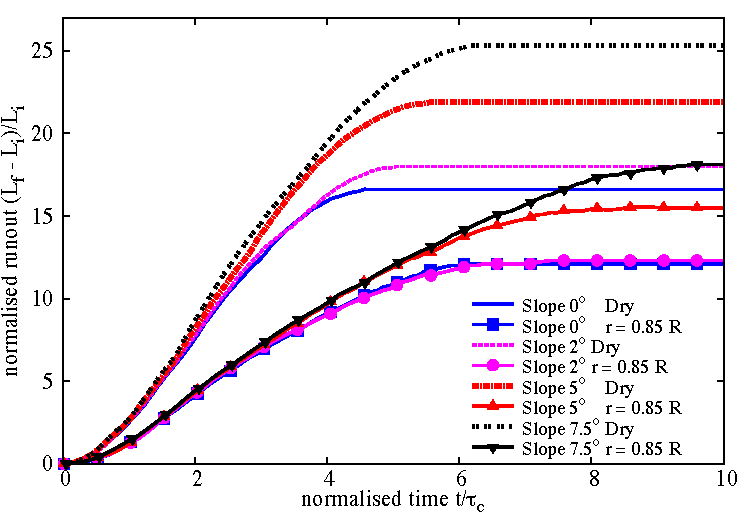
\includegraphics[width=0.9\linewidth]{figs/runout_a6_slope}
\caption{Evolution of run-out for a column collapse in fluid (a = 6).}
\label{fig:Runout_a6_slope}
\end{figure}

\begin{figure}[htbp]
\centering
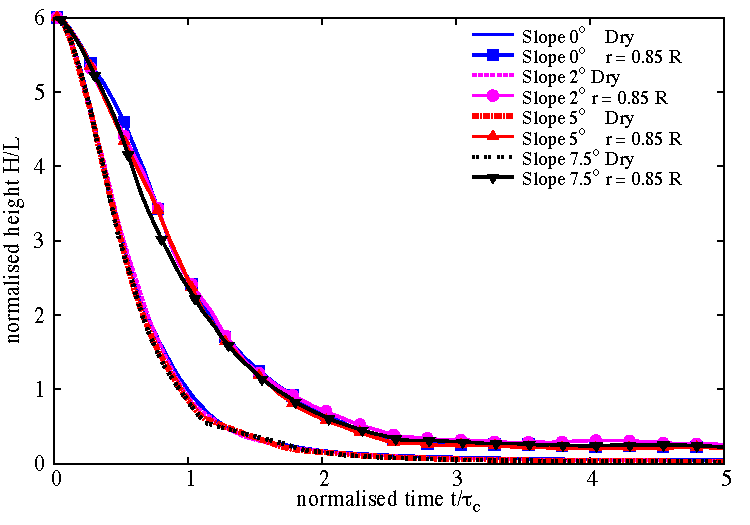
\includegraphics[width=0.8\linewidth]{figs/height_a6_slope}
\caption{Evolution of height with time for a column collapse in fluid (a = 6).}
\label{fig:Height_a6_slope}
\end{figure}

\Cref{fig:KEx_a6_slope,fig:KEy_a6_slope} shows the evolution of the normalised
kinetic energies on different slope angles. The 
amount of kinetic energy available for the flow in the submerged condition 
is almost half that of the dry condition.

\Cref{fig:KEx_a6_slope} shows that in the dry condition, the kinetic energy
available for the flow increases proportionally with the slope angle. However,
in the case of submerged flow slopes 0\si{\degree} and 2\si{\degree},
and 5\si{\degree} and 7.5\si{\degree} have similar kinetic energy evolution.
The longer tail observed in the submerged granular collapse can be attributed to
the formation and migration of eddies and subsequent mass redistribution into heaps.


\begin{figure}[htbp]
\centering
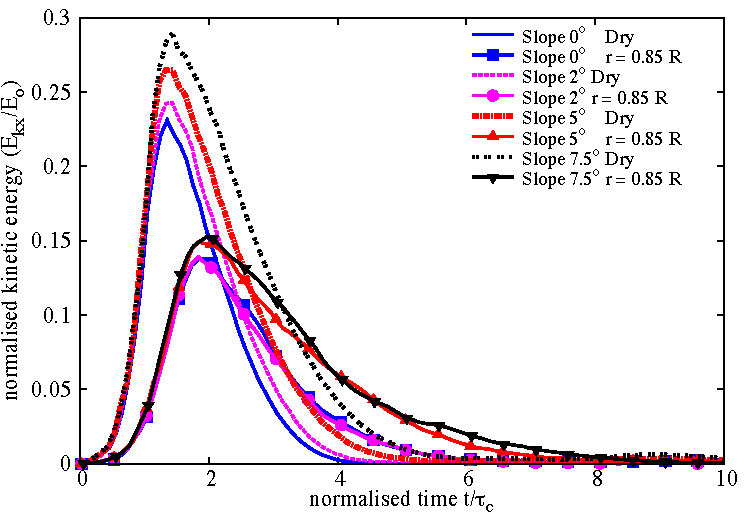
\includegraphics[width=0.9\linewidth]{figs/KEx_a6_slope}
\caption{Evolution of horizontal kinetic energy with time for a granular 
column collapse in fluid (a = 6).}
\label{fig:KEx_a6_slope}
\end{figure}


\Cref{fig:KEx_a6_slope} shows that 
the vertical kinetic energy in the fluid condition dissipates slower, in
comparison to the free-fall release observed in the dry condition. The slower
dissipation is attributed to the viscous drag force experienced by the grains. 
However, the slope angle has negligble effect on the evolution of vertical
kinetic energy in submerged condition. Where as, dry conditions show 
$\approx15\%$ increase in the peak vertical kinetic energy when the slope angle
changes from 0\si{\degree} to 7.5\si{\degree}.

\begin{figure}[htbp]
\centering
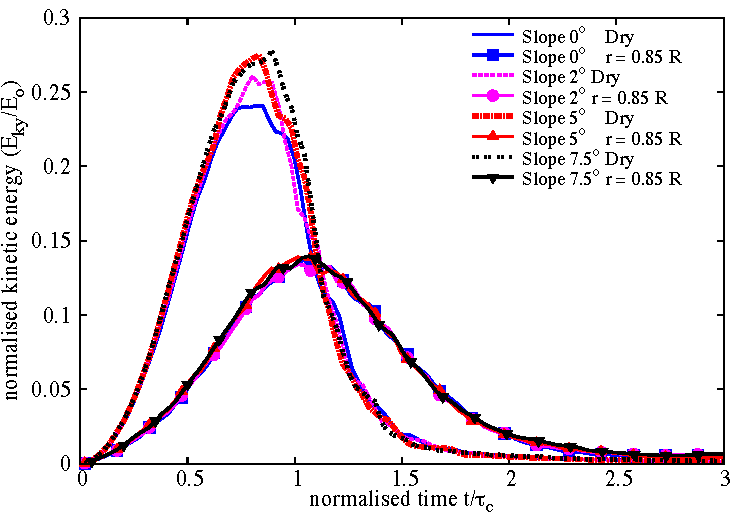
\includegraphics[width=0.8\linewidth]{figs/KEy_a6_slope}
\caption{Evolution of vertical kinetic energy with time for a granular 
column collapse in fluid (a = 6).}
\label{fig:KEy_a6_slope}
\end{figure}

\section{Summary}
The behaviour of tall columns is significantly different from that observed in 
short columns. The slope angle has a strong influence on the number 
and size of eddies during the flow. The eddies interact with the surface of the 
granular flow and forms heaps in front of each vortex. This significantly 
affects the mass distribution and in turn the run-out evolution. Although tall 
cliffs are quite rare in submarine condition, further research is
required to understand the influence of permeability and packing density
on the run-out behaviour.




\section*{Acknowledgements}
The author would like to thank the Cambridge Commonwealth and Overseas Trust
for the financial support to pursue this research.

%
% BibTeX or Biber users please use (the style is already called in the class, ensure 
% that the "woc.bst" style is in your local directory)
% \bibliography{name or your bibliography database}
%
% Non-BibTeX users please use
%
\bibliography{references} 

\end{document}

% end of file template.tex
